
\section{Background}

\subsection{Convolution Operations}

At the convolutional stage, the computational kernel takes as input a batch of 2D multi-channel feature maps and a bank of  2D
multi-channel filters. The computation produces a batch of 2D multi-channel output feature maps with the same batch size as input. To
compute one output feature map, all filters are used to convolve with the same input feature map. Specifically, each filter slides over the
input feature map to perform an elementwise multiplication with the part of input where it is currently located and then sums up the
results across all channels.

\begin{figure}
\centering
  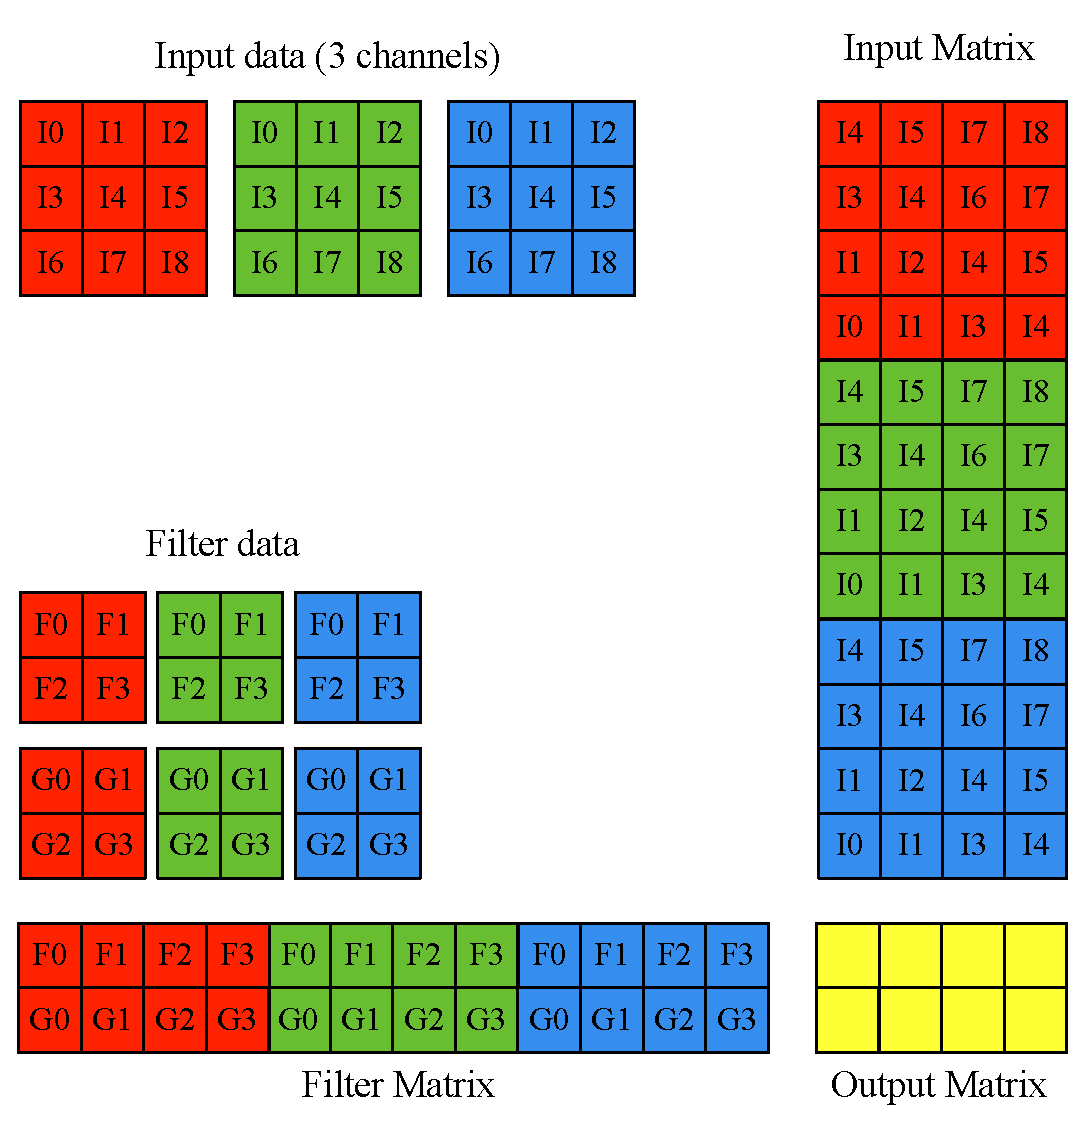
\includegraphics[width=0.75\columnwidth,height=6cm]{./figure/convlowering.eps}
  \caption{An example (reproduced from \cite{ChetlurWVCTCS14}) of converting a simple convolution into matrix multiplications. Here, two filters are used to convolve with a 3-channel input.}
  \label{fig:convlowering}
\end{figure}

{\color{red} Several algorithms, including FFT-based and Winograd-based convolutions, have been proposed to optimize the convolution
operation. All these approaches require to transform 4D tensors into the desired matrix, thus incurring high memory overhead. Figure
\ref{fig:convlowering} illustrates how to translate a simple convolution into matrix multiplications. A filter is typically organised as
4-element tuple, $(batch\_size, chanel\_size, height, width)$. For example, the data dimension of the filter in Figure
\ref{fig:convlowering} is $(2, 3, 2, 2)$. We can see that the transformed filter matrix has the same number of elements as the filter data.
The input data dimension is (1, 3, 3, 3) and 27 elements in total, whereas the input matrix has 48 elements and 44\% of which are redundant
elements. This can incur numberous memory transactions. The experiments (Table \ref{tab:3dtrans}) show that our approach reduce the number
of memory transactions by a factor of 4.4 compared with GEMM-based 3D convolution.}


%\subsection{Overview of Our Approach}
\begin{figure}[t!]
\centering
  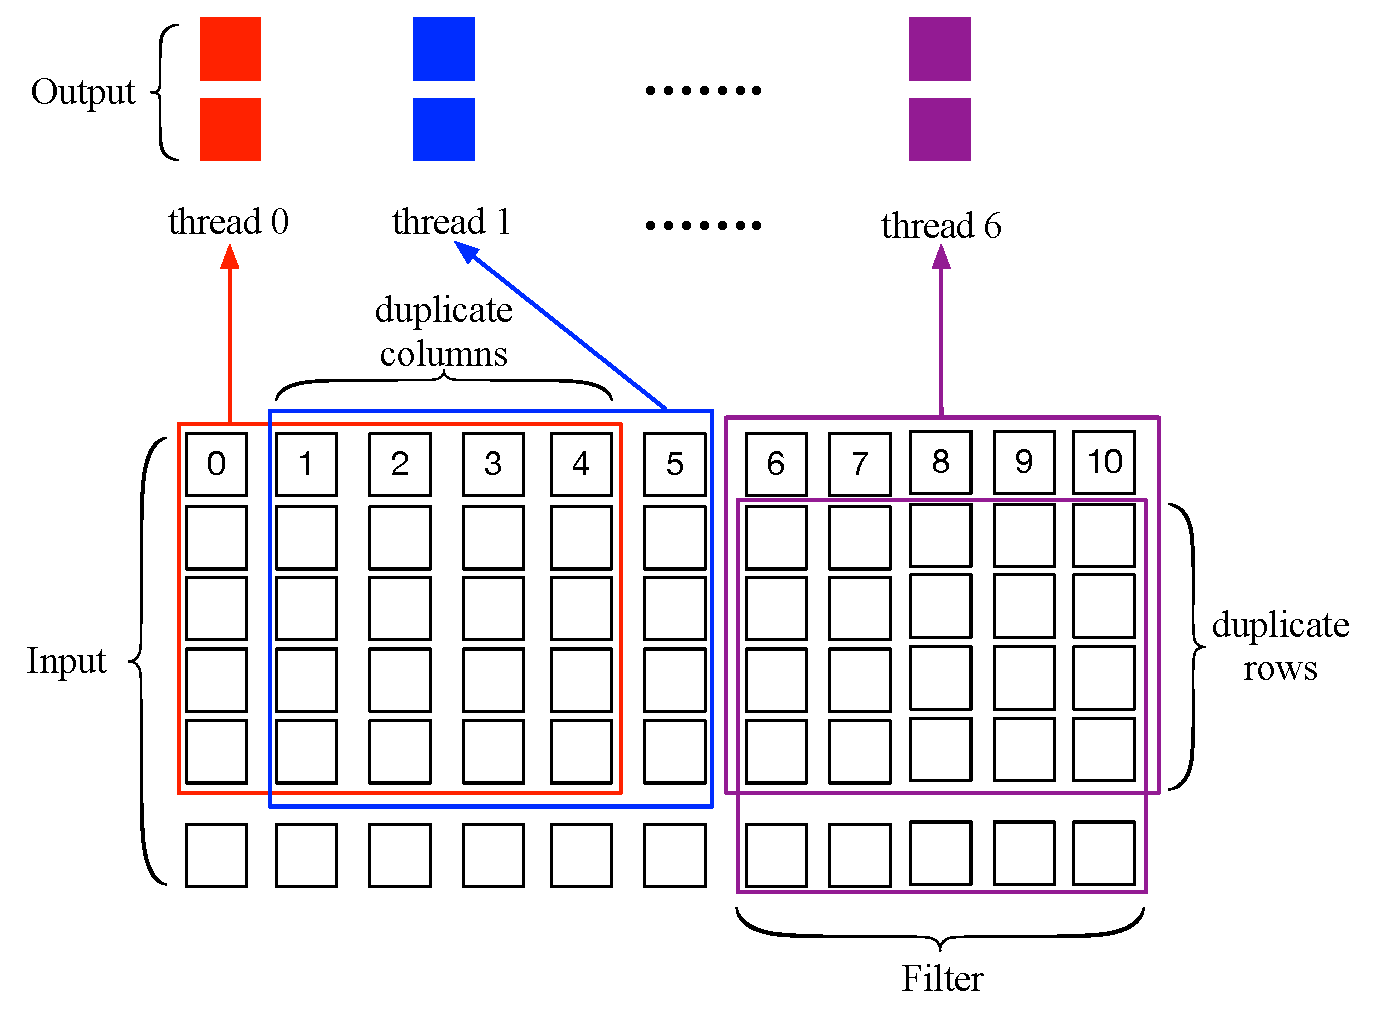
\includegraphics[width=\columnwidth,height=6cm]{./figure/twostrategies.eps}
  \caption{Example of performing 2D convolution using a GPU. Here, the filter size is $5 \times 5$, the input image size is $6 \times 11$
  and the output size is $2 \times 7$. Each thread calculates one column of the output. Assume threads 0 and 1 load the required regions from input
  image with four duplicate columns, and thread 6 loads two overlapped regions from input image and generates four duplicate rows. Numbers in
  the square denote the index of input elements.}
  \label{fig:twostrategies}
\end{figure}
